\documentclass[10pt]{article}

\usepackage{amsmath}                                                                % Math mode $-$ o $$-$$
\usepackage{amssymb}                                                                % Mathematic symbols
\usepackage{mathrsfs}                                                               % Caligraphic letters
\usepackage{amsthm}                                                                 % Theorem-like environments

\usepackage[english]{babel}                                                         % Language (it is important when hyphenating words)
\usepackage[utf8]{inputenc}                                                         % Accented letters and other strange symbols

\usepackage{graphicx}                                                               % Images
\usepackage{float}                                                                  % Puts images where they belong
\usepackage{subcaption}                                                             % Subimages
\usepackage{wrapfig}                                                                % Text and image on the same line
\usepackage{subfiles}                                                               % Subfiles
\usepackage[hidelinks]{hyperref}                                                    % Allows external and internal references
\usepackage[nameinlink]{cleveref}                                                   % Improves internal references
\usepackage[super,square]{natbib}                                                   % Easy bibliography

\usepackage{verbatim}                                                               % Verbatim + multiline comments
\usepackage{anysize}\marginsize{2cm}{2cm}{.5cm}{4cm}                                % Personalizes margins: {L}{R}{U}{D}
\usepackage{bbm}                                                                    % Allows \1
\usepackage{mathdots}                                                               % Rising triple dot symbol
\usepackage{faktor}                                                                 % Fancy rendering of coset sets
\usepackage{tikz-cd}                                                                % Commutative diagrams
\usetikzlibrary{babel}                                                              % Avoids interference between tikz-cd i babel
\usepackage{lipsum}                                                                 % Lorem ipsum dolor sit amet, with \lipsum or \lipsum[1]
\usepackage{todonotes}                                                              % To indicate something is missing
\usepackage[normalem]{ulem}
\usepackage{graphicx}

\usepackage{amsthm}
\usepackage{xcolor}
\usepackage{tcolorbox}
\newtcbox{\mybox}{on line,
  colframe=blue,colback=blue!10!white,
  boxrule=0.5pt,arc=4pt,boxsep=0pt,left=6pt,right=6pt,top=6pt,bottom=6pt}
\usepackage{float}
\usepackage{hyperref}
\hypersetup{
    colorlinks = true,
    filecolor = blue,
    linkcolor = blue,
    urlcolor = blue,
}

\thispagestyle{empty}

\begin{document}
\begingroup
  \centering
  \Huge Wine type and quality determination \\
  \vskip 0.35cm
  \LARGE Intermediate delivery\\
  \vskip 0.25cm
  \large Aleix Torres i Camps, Àlex Batlle Casellas, Luis Sierra Muntané\\[1.5em]
\endgroup


\section{Description and goals of the project.}
Based on \href{http://archive.ics.uci.edu/ml/datasets/Wine+Quality}{this data set} ...

\section{Related previous work.}
This data set has been previously used in various projects, as wine appears to be a frequent topic in examples of classification problems in ML. The first one we cite here is the one provided as a relevant paper, \href{https://www.sciencedirect.com/science/article/pii/S0167923609001377?via\%3Dihub}{Modeling wine preferences by data mining from physicochemical properties}. This paper, as it states in its abstract, proposes a data mining approach to predict human taste preferences on wine, through three different types of regression model: multiple regression, neural networks and support vector machines. This goal is similar to ours, but uses models we cannot comment on for the moment, as they have not been explained in class yet.

Apart from the data set webpage, we have looked for other projects that cite and use this data set. Searching through Kaggle we have found some different kernels operating on this data. Some of these use decision tree-based methods and support vector machines so we are not commenting on them either. Even though, they also use linear and generalized linear models to preliminary test variable significance.

The \href{https://www.kaggle.com/indra90/predicting-white-wine-quality}{first kernel} only uses white wine data. One thing to remark about most of the models used on this kernel is that they binarize the quality of the wines into "good" and "not good" and then use the previous stated models and logistic regression.
In the \href{https://www.kaggle.com/conradws/how-good-is-this-wine-m-l-for-quality-control}{second kernel}, it is remarkable the various ways in which the author tries to gain insight on the data. Initially they use k-Means to cluster data, and then based on the results of this method they visualize the data using a Radial Visualization (RadViz) plot, which we can map into our knowledge as being similar to a biplot. In this way they can observe if there exist any clear tendencies as to variable influence in wine quality. They also pay special attention to anomalies throughout the notebook.
The \href{https://www.kaggle.com/danielpanizzo/red-and-white-wine-quality}{third kernel} we are commenting on is an exploratory data analysis into the data. In this work it is remarkable the univariate distribution exploration, and especially the fact that this is done separately with white and red wine. This indicates that these two variants might need different treatment, which makes our second task (classification into red or white wine) pertinent in the combined data set.

We found some additional data exploration notebooks: namely, \href{https://rstudio-pubs-static.s3.amazonaws.com/57835_c4ace81da9dc45438ad0c286bcbb4224.html}{this one} performs some comparative plots between variables and their correlations, and \href{http://rstudio-pubs-static.s3.amazonaws.com/219996_9cc8cf9f2e7e41fe8912454c3ad2685a.html}{this other one} also investigates univariate, bivariate and multivariate relationships between variables.
\section{Data exploration.}
First of all, the dataset is given into two different tables, on for red wine and the other for white. Then we decided to perform the union and \textbf{obtain an unique dataset}. After that, we extracted the two targets vectors. The first one, wine.type, determine if the wine is red or white and the second one, wine.quality, is the value given by the oenologist. \\ \ \\
After some exploration, we detected something that we didn't expect: some rows have the exact same values in all the variables. So we concluded that there are \textbf{duplicated rows} in the dataset. So we went back and decided to delate them (only duplicated). But a major problem was found, 2 rows were at the same time in the two original datasets. In this situation we decided, for now, to delate them from both. Because we don't know from where they were and we still have a lot of others rows. \\ \ \\
Now, we were interested in the \textbf{dimensions of the dataset}. So we observed there are 5318 rows and 11 input variables. From these rows, 1357 are red wines and 3959 white. And the table of wine quality with respect to the numbers of rows with that value is:
\begin{table}[H]
\caption{Number of wines of each quality}
\centering
\begin{tabular}{|c|c|c|c|c|c|c|c|}
\hline
wine quality  & 3  & 4   & 5    & 6    & 7    & 8   & 9 \\ \hline
num. of wines & 30 & 206 & 1751 & 2323 & 855  & 148 & 5 \\ \hline
\end{tabular}
\end{table}
\ \\
Then, from these information we may extract some conclusions. The first one is that not all possible marks ([0,10]) of the wine were given. And more important, \textbf{the dataset is unbalanced} with respect to wine type and wine quality. There are the triple of white wines than red and most of the marks are 6 and 5 then 7 and the others ones have a very small amount. \\ \ \\
The next thing we did is to care about \textbf{missing values}. After some exploration using summary and histograms, the conclusion is that there are not missing values. Although a variable was suspicious, that was citric.acid, because it has a very large amount of 0 values, most of them coming from the white wines. But, as it is a supplement used as a natural preservative or a flavour potential, we may think that some wines have not citric acid. \\ \ \\
In the review of the data, some \textbf{outliers} were found. Such as a wine with 1.66 in citric.acid, while the 3rd quartile is 0.4, or another with residual sugar 65.8, while the 3rd quartile is 7.5. For the moment we decided to keep them but may be we delate them in the future. \\ \ \\
So then, we perform a \textbf{particular analysis of each variable}. We saw that all the variables of the new dataset are numerical, therefore we can perform computations over them. But two variables seems to be discrete (free.sulfur.dioxide and total.sulfur.dioxide). One of the target variables is also discrete and the other is a factor of two elements. \\ \ \\
We start plotting the \textbf{histograms}, with different colors for each wine type. We detect that for fixed.acidity, volatile.acidity and citric acid, the two wine types have different behaviours: the white type is more like a normal distribution, while the red is more uniform. These variables have in common that all of them are related to acidity so may be in the future we perform a join variable. \\
\begin{figure}[H]
\centering
\caption{Histograms of 3 variables}
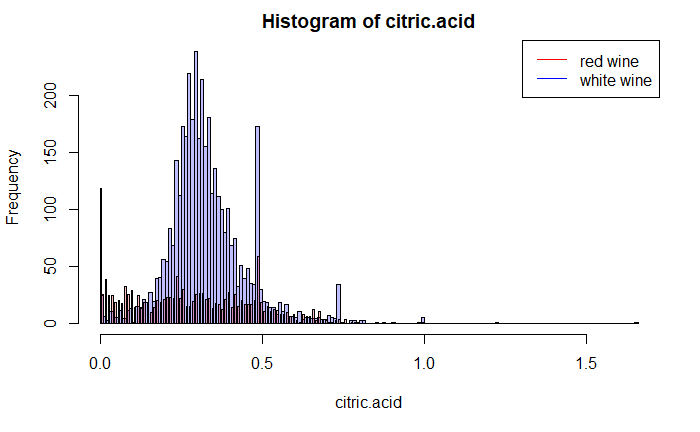
\includegraphics[scale=0.3]{histogram_of_citricacidity}
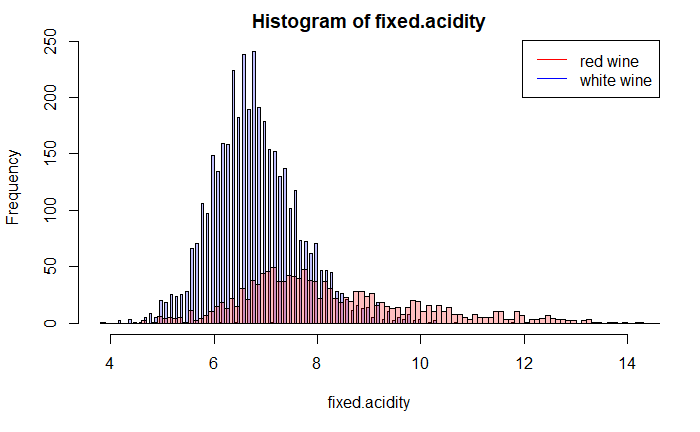
\includegraphics[scale=0.3]{histogram_of_fixedacidity}
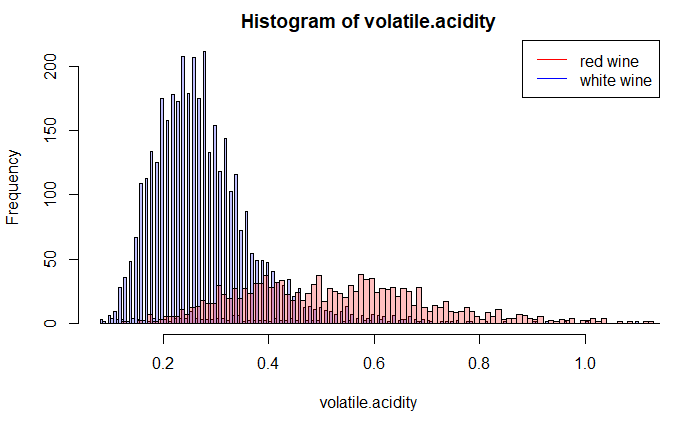
\includegraphics[scale=0.3]{histogram_of_volatileacidity}
\end{figure}
\ \\
The second thing we detected is that the variable residual.sugar has a lot of small entries a less from the others so we considered to apply logarithmic function and see the result. There is a clear improve, but something interesting was discovered. The red wine can be modeled as a unique normal distribution but the white wine as two, as there are two density regions with a separation between them. So we can see the logarithm of the residual.sugar as a \textbf{variable extracted} that can be useful.
\begin{figure}[H]
\centering
\caption{Histograms of a residual.sugar and its logarithm}
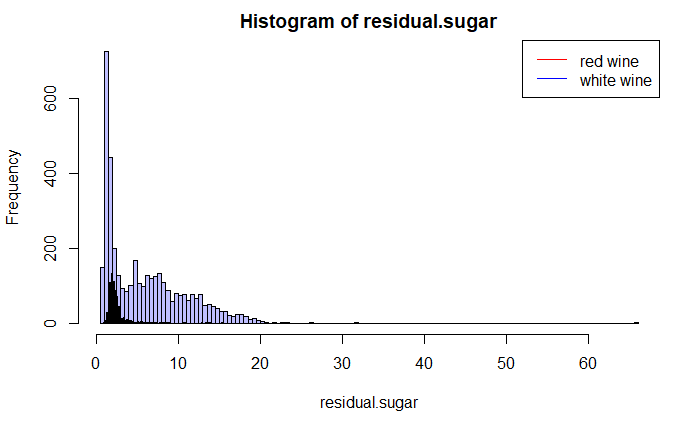
\includegraphics[scale=0.4]{histogram_of_residualsugar}
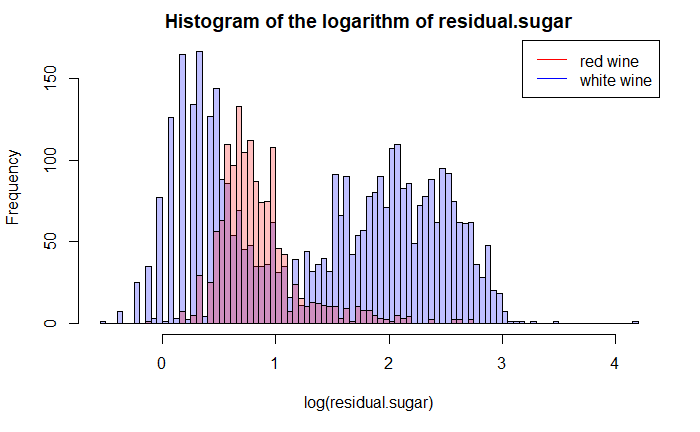
\includegraphics[scale=0.4]{histogram_of_log_residualsugar}
\end{figure}
\ \\
Finally, the other ones have a similar shape independent of the wine type, but normally with different means. Something that we be useful when we will perform classification. And will be relevant for the regression model to differentiate them as factors. Here some of the others histograms: \\
\begin{figure}[H]
\centering
\caption{Histograms of 4 variables}
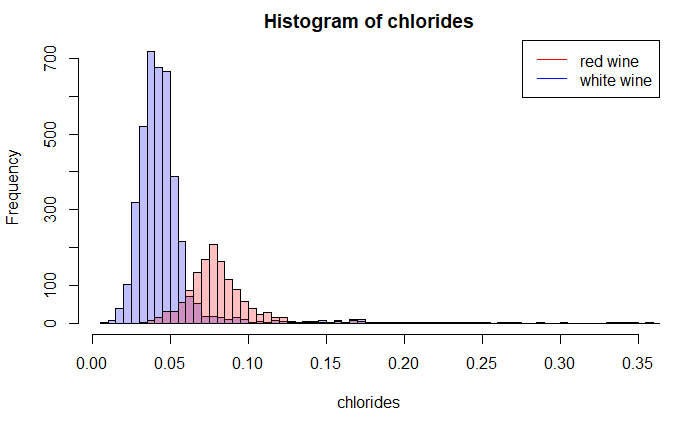
\includegraphics[scale=0.4]{histogram_of_chlorides}
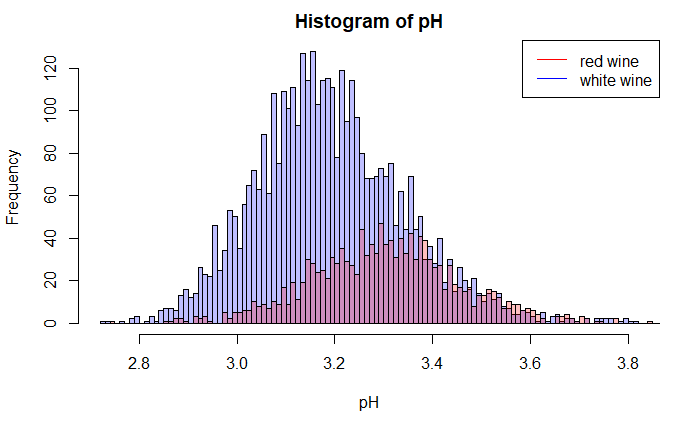
\includegraphics[scale=0.4]{histogram_of_pH}
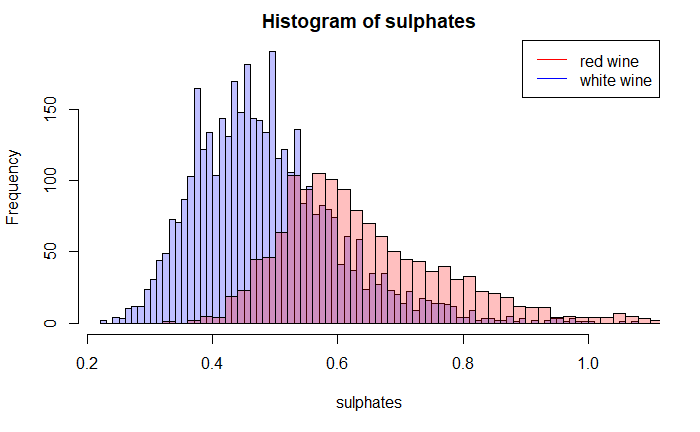
\includegraphics[scale=0.4]{histogram_of_sulphates}
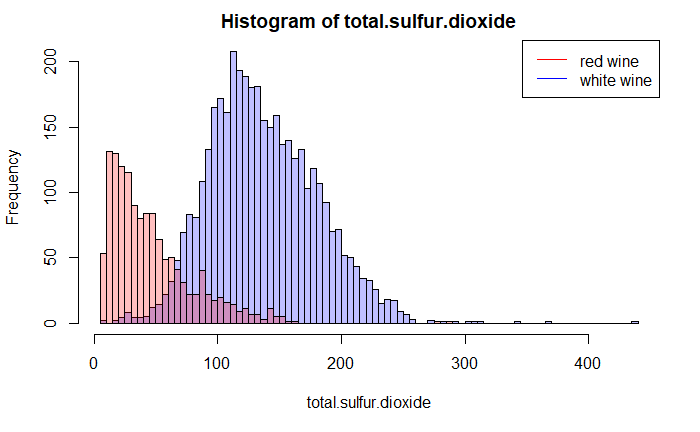
\includegraphics[scale=0.4]{histogram_of_totalsulfurdioxide}
\end{figure}
\ \\
The next thing we did is to perform a PCA, because it can help us to visualize the data and start seeing which variables are more relevant or less. We made the following biplot, where the first two components explain 50\% of the variability. \\
\begin{figure}[H]
\centering
\caption{PCA biplot}
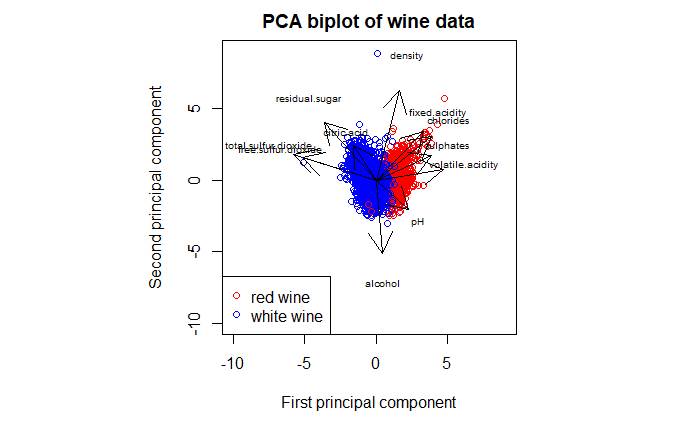
\includegraphics[scale=0.75]{PCA_biplot}
\end{figure}
\ \\
As the two groups seems to be separate into the horizontal edge, it seems that the density and alcohol variables not explain the diferents between the groups. And variables such as total.sulfur.dioxide or volatile.acidity do. In the PCA we can also see that some variables are very correlated, for example, total.sulfur.dioxide and free.sulfur.dioxide or residual.sugar and citric.acid. There is a last thing we observed, the outliers. There are points that are not only far from the others in one variable, so they are in a multiple of them. We will consider to remove them or not.   \\ \ \\

\section{Modelling methods considered.}

\section{Preliminary results.}

\section{Future approaches.}

\section{References:}
\begin{enumerate}
  \item Web page where the data set can be found:

  \href{http://archive.ics.uci.edu/ml/datasets/Wine+Quality}{ http://archive.ics.uci.edu/ml/datasets/Wine+Quality}

  \item Relevant paper (a previous approach):

  \href{https://www.sciencedirect.com/science/article/pii/S0167923609001377?via\%3Dihub}{ https://www.sciencedirect.com/science/article/pii/S0167923609001377?via\%3Dihub}


\end{enumerate}



\end{document} 